\documentclass[ThesisDJ.tex]{subfiles}

\begin{document}
    Dieser Abschnitt dokumentiert die Durchführung des Projektes und zeigt dabei getroffene Maßnahmen zur Überwachung und Steuerung des Projektfortschrittes auf.\\
    Ziel ist es dabei, sicherzustellen, dass Abweichungen von der erfolgten Projektplanung und den damit in Verbindung stehenden Zielen so früh wie möglich erkannt 
    werden und ein Gegensteuern möglich ist \cite[S.~55ff]{riedl_management_2019}. In Kombination mit einer strukturierten Projektdurchführung, die die Umsetzung von 
    getroffenen Maßnahmen gewährleistet, soll der Projekterfolg messbar und kontrollierbar werden.

    \subsection{Theoretische Grundlagen des Projektcontrollings}
    Projektcontrolling beschreibt Maßnahmen, Regeln und Abläufe, die sicherstellen sollen, dass Projektziele
    erreicht werden \cite{kerzner_project_2022} \cite[S.~189]{kuster_handbuch_2022}. Dabei unterscheidet sich die konkrete Ausprägung 
    je nach verwendetem Vorgehensmodell. Bei einer traditionellen Vorgehensweise ist Projektcontrolling ein eigenständiger Prozess im Ablauf, welcher
    als Zyklus mit drei Etappen visualisiert werden kann, wie bspw. in Abbildung \ref{fig:controlling} zu sehen ist \cite[S.~191]{kuster_handbuch_2022}.

    \begin{figure}
        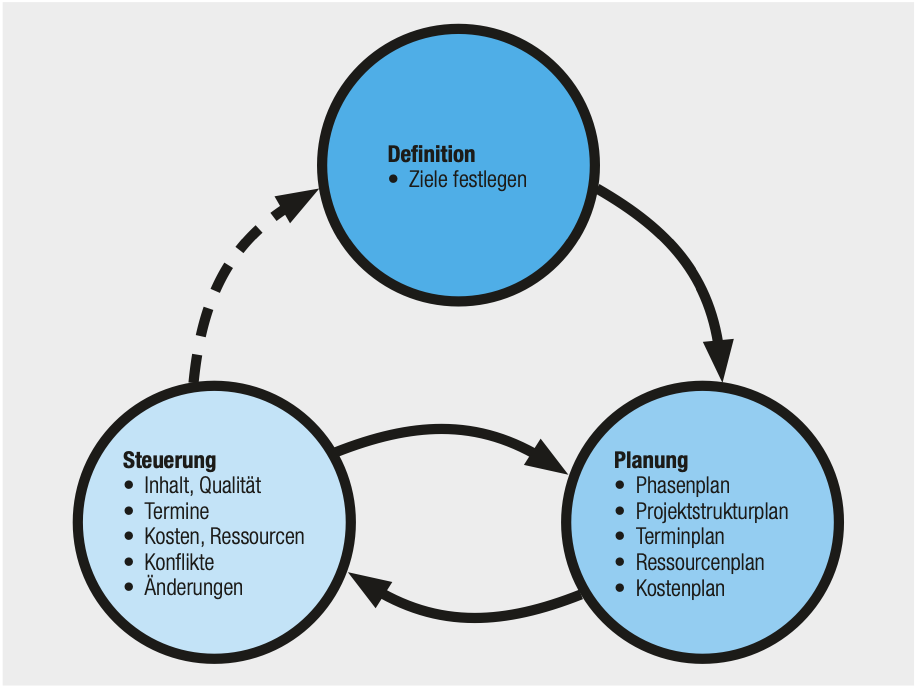
\includegraphics[scale=0.8]{controlling.png}
        \centering
        \caption{Die drei Etappen des Projektcontrollings}
        \label{fig:controlling}
    \end{figure}

    Der Controllingzyklus beginnt mit der Definitionsphase, in der eine korrekte und möglichst vollständige Vereinbarung zwischen dem Projektteam und dem 
    Auftraggeber ausgearbeitet wird. Diese Vereinbarung stellt dann die Basis für die konkrete Projektplanung, bei der im traditionellen Vorgehensmodell
    verbindliche Dokumente erstellt werden, welche für die Steuerung des Projektes als Maßstab herangezogen werden. Die eigentliche Steuerung 
    vergleicht dann kontinuierlich den Soll-Zustand mit dem aktuellen Ist-Zustand. Bei Abweichungen wird ein neuer Durchlauf des Zykluses angestoßen, bei dem die 
    Abweichungen in der Planungphase addressiert werden. Dadurch entstehen neue Planungsdokumente, welche dann für das weitere Steuern herangezogen werden. Dieser Zyklus wiederholt sich 
    bis zum Ende des Projektes \cite[S.~217]{dechange_projektmanagement_2024}. \\

    Im Gegensatz zum klassischen Projektcontrolling, das als ein klar abgegrenzter und zyklischer Prozess mit definierten Phasen (Definition, Planung, Steuerung) verstanden wird, 
    zeichnet sich das agile Controlling durch eine flexible und iterative Vorgehensweise aus. 
    Während im traditionellen Modell die Steuerung in regelmäßigen, aber längeren Intervallen (z.B. in Form von Soll-Ist-Vergleichen) erfolgt,
    sind im agilen Umfeld die Controllingmaßnahmen in den gesamten Arbeitsprozess integriert und erfolgen in kürzeren, oft iterativen Zyklen.
    Typische Werkzeuge für agiles Controlling sind Element wie Daily Standups, Reviews und Retrospektiven. Diese Werkzeuge kommen als feste Bestandteile 
    des agilen Arbeitsablaufes vor. Ein eigenständiger Zyklus wie bei traditionellen Vorgehensmodellen, wird hier nicht angewendet.

    \subsection{Methoden zur Erfassung des Projektfortschritts}
    Es gibt verschiedene Methodiken, mit denen im Rahmen des Projektcontrollings eine Fortschrittsbewertung durchgeführt werden kann.
    In diesem Abschnitt werden exemplarisch einige Methodiken vorgestellt, um im Anschluss aufzuzeigen, wie mit Ihnen eine Steuerung des Projektes durchgeführt 
    wurde.

    \subsubsection{Earned-Value-Analyse}
    Die Earned-Value-Analyse ist eine Methode zur Fortschrittsbewertung von Projekten, welche auf dem sogenannten \emph{magischen Dreieck} basiert. Dieses 
    besteht aus den drei Ecken \emph{Scope}, \emph{Kosten} und \emph{Zeit}, wie in Abbildung \ref{fig:magic_tri} zu sehen ist \cite[S.~84]{kuster_handbuch_2022}.
    In einer Earned-Value-Analyse wird dabei der \emph{erreichte Mehrwert} berechnet, d.h. wie viel konnte 
    in einer Zeitperiode vom Projekt fertiggestellt. Dies wird in Verhältnis zu dem im Voraus geplanten Aufwand und den verursachten Kosten 
    gesetzt. Wichtig dabei ist, dass nur vollständig abgeschlossene Arbeitspakete bzw. Meilensteine berücksichtigt werden.
    
    \begin{figure}
        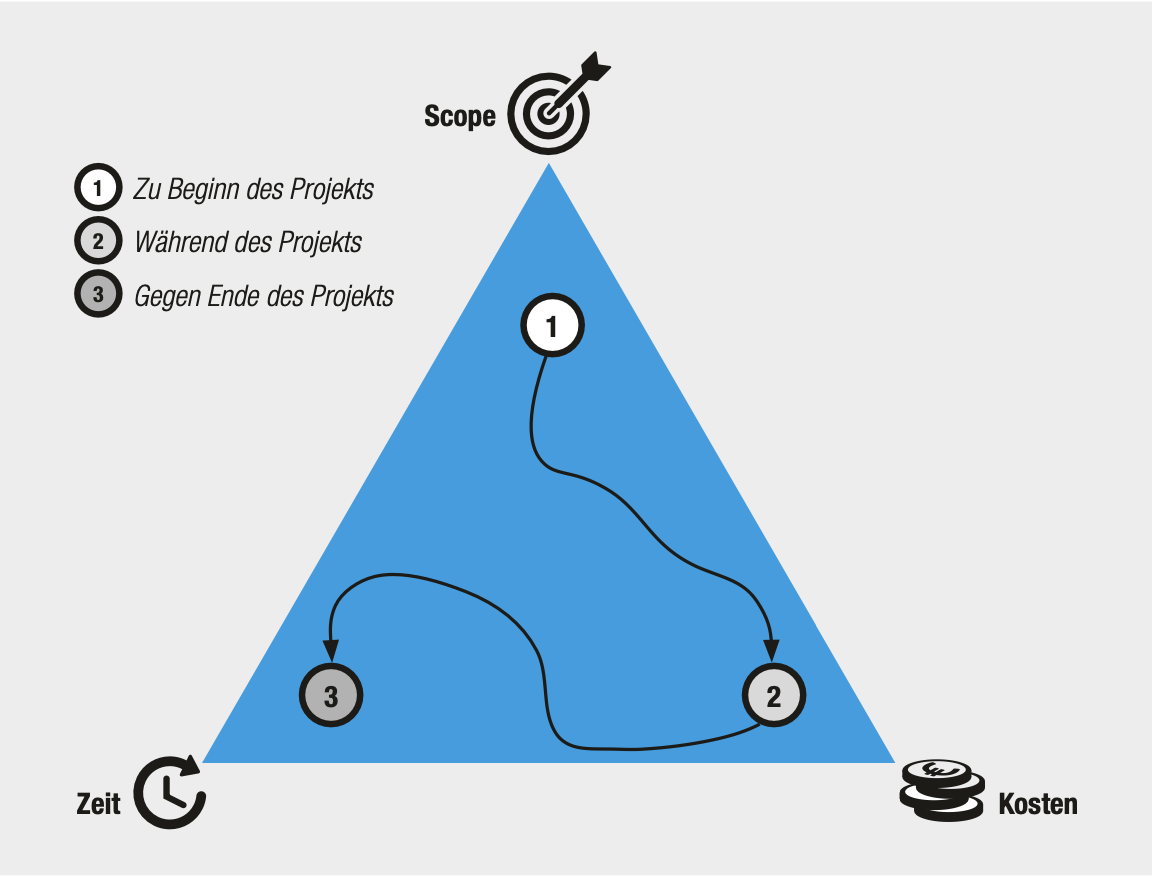
\includegraphics[scale=0.5]{magic_tri.png}
        \centering
        \caption{Das magische Dreieck}
        \label{fig:magic_tri}
    \end{figure}

    \subsubsection{Meilensteintrendanalyse}
    Die Meilensteintrendanalyse verwendet die Meilensteinplanung des Projektes zur Beurteilung des Projektfortschritts.
    Damit eine sinnvolle Anwendung möglich ist, müssen ausreichend Meilensteine und Fälligkeitstermine im Voraus definiert sein.
    Ein Vortiel der Meilensteintrendanalyse ist, dass sich die zeitliche Entwicklung in Form einer Prognosekurve zeigt, welche 
    zur Abschätzung für den zukünftigen Verlauf verwendet werden kann. Der Mehrwehrt in dieser Methode liegt in der 
    übersichtlichen Darstellung von erreichten Mehrwerten in Kombination mit noch bevorstehenden Arbeiten. Eine bespielhafte Darstellung ist in Abbildung
    \ref{fig:mta} zu finden \cite[S.~192]{kuster_handbuch_2022}.

    \begin{figure}
        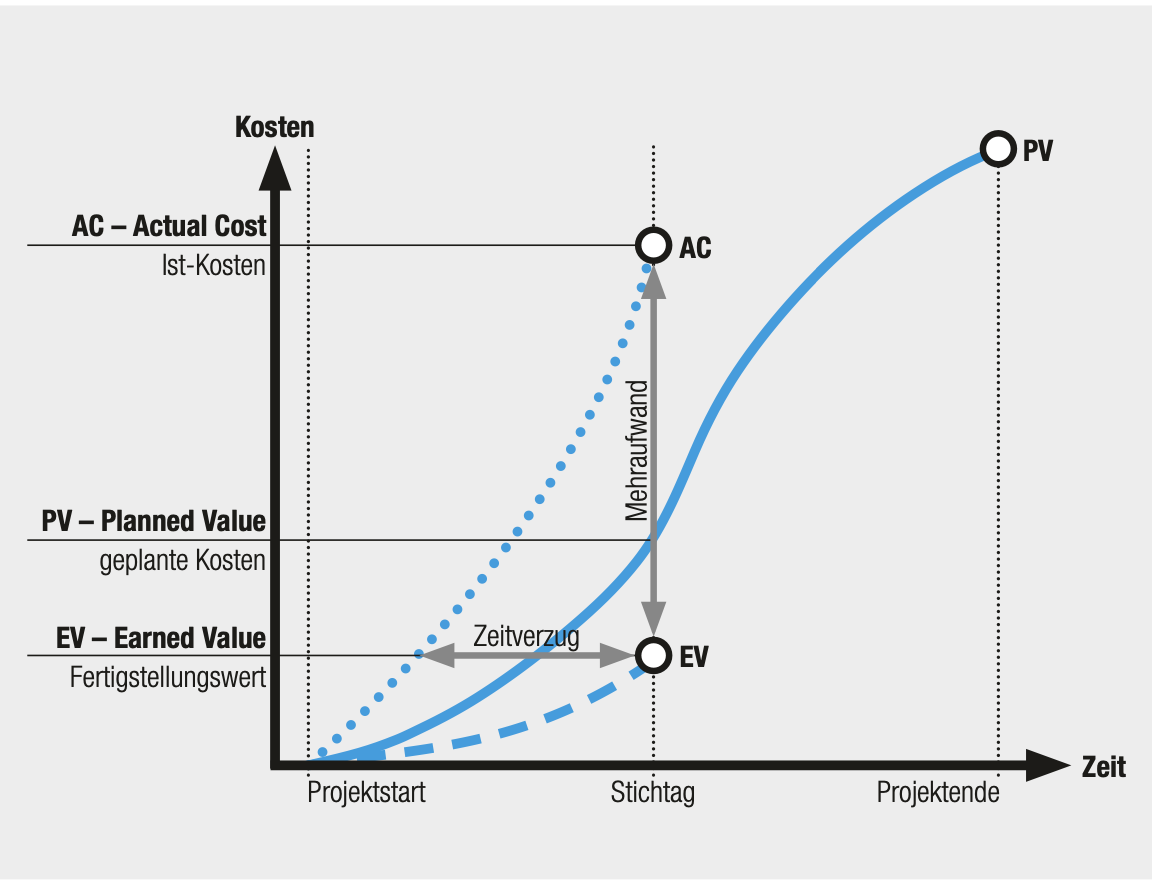
\includegraphics[scale=0.5]{mta.png}
        \centering
        \caption{Beispiel einer Meilensteintrendanalyse}
        \label{fig:mta}
    \end{figure}

    \subsubsection{Burndownchart}
    Die Burndown-Chart ist eine im agilen Projektmanagement besonders beliebte Methode zur Fortschrittsüberwachung. 
    Auf der vertikalen Achse werden die kumulativ verbleibenden Aufwände im Backlog dargestellt, während die horizontale Achse die Anzahl der verbleibenden Arbeitstage zeigt. 
    Eine Ideallinie, die von oben links nach unten rechts verläuft, gibt an, welche Aufwände an den jeweiligen Tagen erbracht werden müssten, um das gesetzte Ziel termingerecht zu erreichen. 
    Der tatsächliche Projektverlauf wird in derselben Grafik eingezeichnet. Im optimalen Fall nähert sich der reale Verlauf kontinuierlich der Ideallinie an. 
    Die Burndown-Chart erweist sich dabei insbesondere für kurze Zeiträume, wie beispielsweise während eines Sprints, als ein effektives Instrument zur Überwachung des Fortschritts.
    Eine beispielhafte Burndownchart ist in Abbildung \ref{fig:burndown} zu finden \cite[S.~279]{dechange_projektmanagement_2024}.

    \begin{figure}
        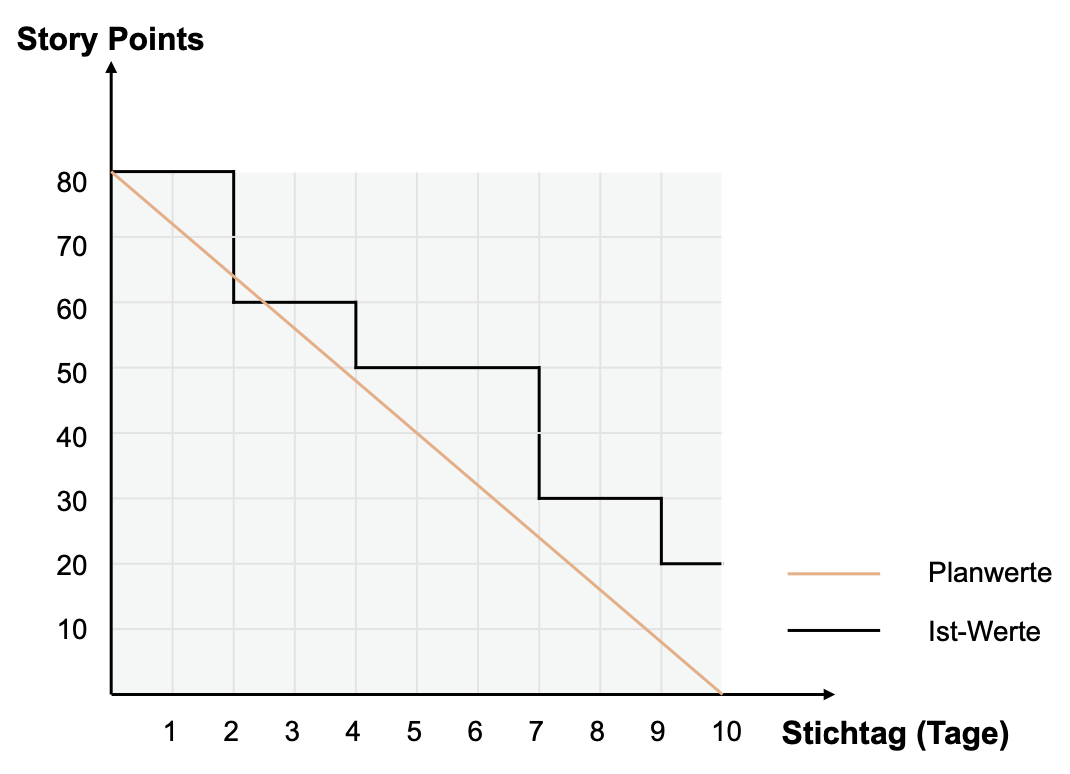
\includegraphics[scale=0.5]{burndown.png}
        \centering
        \caption{Beispielhafte Burndownchart}
        \label{fig:burndown}
    \end{figure}

    \subsection{Controlling im Laufe des Projektes}
    In diesem Abschnitt werden die tatsächlich angewendeten Methoden zur Überwachung und Steuerung des 
    Projektes examplarisch gezeigt. Dadurch wird aufgezeigt, wie das Projekt während der Durchführung gesteuert wurde 
    und wie auf aufkommende Abweichungen reagiert wurde.\\
    Zum Steuern des Projekts wurde sich mit einem Burndownchart beholfen. Die vertikale Achse zeigt dabei die Personenstunden. Die Horinzontale den Zeitpunkt im Projekts.\\
Dargestellt sind hier zwei Graphen. Der blaue Graph zeigt die Ideallinie. Diese gibt an welche Aufwände im Idealfall zu einem bestimmten Datum erledigt sein müssen. Die orangene Linie gibt den tatsächlich verbleibenden Aufwand im Projket an. Untypisch ist der große Zeitraum über den sich das Burndownchart erstreckt. Begründet wird dies in diesem Fall dadurch, dass die Mitarbeitenden nur jeweils einmal die Woche am Projekt gearbeitet haben und dadurch in diesem Zeitraum verhältnismäßig wenige Arbeitspakete bearbeitet werden mussten.

\begin{figure}
    \centering
    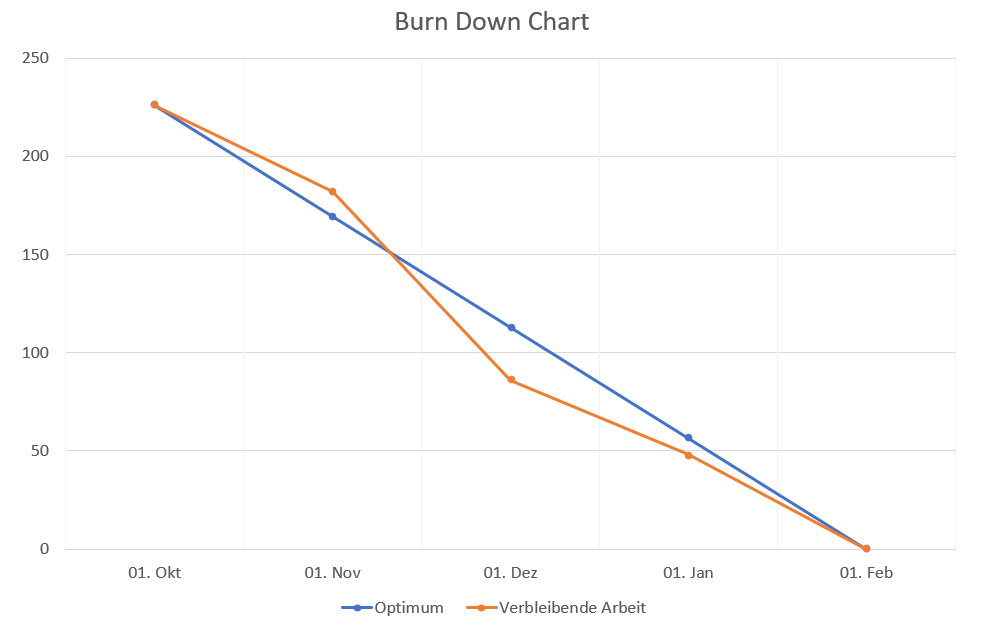
\includegraphics[width=\linewidth]{burnDownChart.png}
    \caption{Burndownchart des untersuchten Projekts}
    \label{fig:realburndown}
\end{figure}

\subsubsection{Projektverlauf}

Anhand des Burndowncharts wird sichtbar, das zu Beginn des Projekts der real erbrachte Aufwand nah an der Ideallinie liegt.\\
In der zeitlichen Mitte des Projekts wurde mehr Aufwand erbracht als die Ideallinie vorgibt.\\
Von der Mitte des Projekts bis zum Ende näherte sich die Verbleibende Arbeit der Ideallinie von unten an.
Die Abweichung vom Ideal ist durch die Verteilung der Arbeitspakete zu erklären. Zu Beginn des Projektes wurde einiges an Zeit in organisatorische Tätigkeiten investiert. Auf diese Tätigkeiten hatten die Projektmitarbeiter nur begrenzt Einfluss. In der Zeit von November bis Januar wurde sich mit dem Kern des Projekts befasst. Diese Arbeit lag allein in der Hand der Studenten. Durch die örtlichen Gegebenheiten war während dieses Abschnitts eine direkte Kommunikation möglich und es musste nicht lange auf Antworten gewartet werden. Zudem sind keine Risiken eingetreten wie Krankheit oder anderweitige Ausfälle. Das Projekt konnte also ungestört voranschreiten. 
In der Phase des Projektabschlusses wird der Kreis der Beteiligten wieder größer und die Kommunikation umschließt wieder mehr Personen, beispielsweise in der Absprache für einen Übergabetermin. Zudem wird die zeitliche Verfügbarkeit der Projektmitarbeitenden gegen Ende des Projektes zunehmend von anderen Projekten und Tätigkeiten vereinnahmt. Dies hat zur Folge, dass das Projekt gegen Ende deutlich langsamer voranschreitet, als zuvor.

\end{document}
